\documentclass[IB,BIB]{TFUOC}%IB: CASTELLANO, CAT: CATALÁN, ENG: ANGLÈS

%Introducción de datos del trabajo
\title{Predicción jerárquica de demanda en retail mediante modelos basados en árboles y redes LSTM con reconciliación jerárquica e interpretabilidad SHAP: aplicación al dataset M5 Forecasting (Walmart)}
\titcrt{Predicción jerárquica de demanda} %Título corto que aparecerá a la cabecera
\author{Tatyana Silchenko Kozyrieva}
\date{22 de marzo de 2026}


\nomPDC{Aarón Montero Montero}
\nomPRA{Susana Acedo}
\titulac{Máster en Ciencia de Datos}
\area{Área 1}

\idioma{Castellano}
\credits{12}
\parcla{time series forecasting; retail demand; machine learning; XGBoost; LightGBM; SHAP values; M5 Forecasting; interpretability; hierarchical forecasting; forecast reconciliation}

\licenc{ccBy}
%Posibles licencias
%ccByNcNd
%ccByNcSa
%ccByNc
%ccByNd
%ccBySa
%ccBy
%GNU
%copyright


%%%%%%%%%%
% Resumen en el idioma

\abstractidioma{
Este Trabajo Final de Máster desarrolla un sistema de predicción jerárquica de demanda en retail utilizando el dataset M5 Forecasting – Walmart, caracterizado por su estructura multinivel y su elevada dimensionalidad temporal y categórica.
El proyecto implementará y evaluará modelos basados en árboles de decisión (Random Forest, XGBoost y LightGBM) para la predicción simultánea de múltiples series temporales, priorizando eficiencia computacional y capacidad de generalización.
De forma complementaria, se implementará un modelo basado en redes neuronales recurrentes (LSTM) con el objetivo de comparar su capacidad para capturar dependencias temporales de largo plazo frente a los modelos tabulares.
Se incorporará reconciliación jerárquica mediante el método MinT (Minimum Trace), utilizando Bottom-Up como referencia comparativa, con el objetivo de garantizar coherencia estructural entre los distintos niveles de agregación del dataset.
Se incorporará un análisis de interpretabilidad mediante SHAP para cuantificar la contribución marginal de las variables explicativas y analizar la estabilidad del modelo en distintos niveles jerárquicos.
El trabajo se orienta a construir una solución reproducible, evaluable mediante métricas estándar del dominio (RMSE, MAE y WRMSSE, métrica oficial del dataset M5) y aplicable a escenarios reales de planificación de inventario.
}

% Resumen en inglés.
\abstractenglish{
This Master's Thesis develops a hierarchical demand forecasting system for the retail sector using the M5 Forecasting – Walmart dataset, characterized by its multi level structure and high temporal and categorical dimensionality. The project will implement and evaluate tree based models (Random Forest, XGBoost, and LightGBM) for the simultaneous prediction of multiple time series, prioritizing computational efficiency and generalization capability.
In addition, a recurrent neural network model (LSTM) will be implemented to compare its ability to capture long term temporal dependencies against tabular models. Hierarchical reconciliation will be incorporated through the MinT (Minimum Trace) method, using Bottom Up as a comparative baseline, with the aim of ensuring structural coherence across the different aggregation levels of the dataset.
An interpretability analysis using SHAP will be included to quantify the marginal contribution of explanatory variables and assess model stability across hierarchical levels. The work aims to build a reproducible solution, evaluated through standard domain metrics (RMSE, MAE, and WRMSSE—the official metric of the M5 dataset), and applicable to real world inventory planning scenarios.
}

\usepackage{graphicx}
\usepackage{pdflscape}
\usepackage{soul}

\usepackage{longtable}
\usepackage{tabularx}
\renewcommand{\tablename}{Tabla}
\addto\captionsspanish{\renewcommand{\tablename}{Tabla}}
\usepackage{booktabs}
\usepackage{longtable}
\usepackage{array}
\usepackage{hyperref}
\usepackage[T1]{fontenc}

\begin{document}
\estructura
\tableofcontents


\chapter{Definición del TFM}

\section{Descripción de la propuesta y justificación del interés}

La predicción de demanda condiciona directamente decisiones de
reposición, planificación logística y optimización de inventarios. En
entornos retail con alta granularidad y múltiples niveles jerárquicos,
el modelado requiere estructuras que equilibren precisión y
escalabilidad.

El dataset M5 constituye un benchmark relevante por su complejidad
estructural y por incorporar información temporal, categórica y de
calendario, lo que permite abordar el problema desde una perspectiva de
feature engineering intensiva.

Los modelos basados en árboles resultan especialmente adecuados en este
contexto por su capacidad para modelar relaciones no lineales, su
robustez ante escenarios de alta dimensionalidad, su buen rendimiento en
entornos tabulares con variables derivadas y su mayor eficiencia
computacional frente a modelos puramente secuenciales.

La incorporación de SHAP permite analizar coherencia y estabilidad del
modelo, facilitando su interpretación en un entorno profesional donde la
explicabilidad es un requisito operativo.

\section{Motivación personal}

La elección de esta temática responde a un doble interés. Por un lado,
profesional, dado que la predicción de demanda y la modelización de
datos complejos constituyen áreas estratégicas dentro de la ingeniería
de datos y la analítica avanzada. Por otro, académico, al permitir
profundizar en técnicas de machine learning aplicadas a series
temporales jerárquicas, así como en metodologías de evaluación rigurosas
e interpretabilidad de modelos.

El dataset M5 Forecasting -- Walmart ofrece un entorno de alta
complejidad estructural que permite abordar un problema realista y
exigente, alineado con escenarios profesionales actuales.

Asimismo, el trabajo permite analizar el equilibrio entre complejidad
modelística y eficiencia computacional, cuestión relevante tanto desde
la perspectiva técnica como estratégica.

\newpage

\section{Hipótesis}

Los modelos basados en árboles, combinados con técnicas de
reconciliación jerárquica, pueden ofrecer un rendimiento competitivo
frente a modelos LSTM en la predicción jerárquica de demanda,
manteniendo un menor coste computacional y proporcionando un mayor grado
de interpretabilidad mediante el uso de SHAP.

\section{Objetivos}

\subsection{Objetivo principal}

Desarrollar y evaluar un sistema de predicción jerárquica de demanda
aplicado al dataset M5 Forecasting -- Walmart, comparando modelos
basados en árboles y redes LSTM, incorporando reconciliación jerárquica
mediante MinT e interpretabilidad mediante SHAP, con el fin de analizar
su rendimiento predictivo y su eficiencia computacional en un contexto
multinivel.

\subsection{Objetivos secundarios}

\begin{itemize}
\item
  Preparar y transformar el dataset M5 para su uso en modelos basados en
  árboles.
\item
  Entrenar y comparar modelos como Random Forest, XGBoost y LightGBM.
\item
  Evaluar el rendimiento mediante métricas adecuadas (RMSE, MAE y
  WRMSSE, métrica oficial del dataset M5).
\item
  Analizar la importancia y contribución de las variables mediante SHAP
  values.
\item
  Integrar la reflexión sobre sostenibilidad, ética y diversidad (CCEG).
\item
  Implementar técnicas de reconciliación jerárquica (Bottom-Up y MinT)
  sobre las predicciones generadas por los distintos modelos, con el fin
  de garantizar coherencia estructural entre niveles agregados y
  desagregados.
\item
  Desarrollar un modelo LSTM multiserie para comparar su rendimiento
  frente a los modelos basados en árboles.
\item
  Analizar el coste computacional y la eficiencia relativa de los
  distintos enfoques modelísticos.
\item
  Desarrollar un panel de visualización en Power BI para comunicar
  resultados y facilitar la interpretación de las predicciones y
  explicaciones del modelo.
\end{itemize}

\newpage
\section{Metodología}

\subsection{Revisión del estado del arte}

La revisión del estado del arte abordará las principales técnicas de
forecasting aplicadas al sector retail, con especial atención a modelos
basados en árboles adaptados a series temporales y a los enfoques
contemporáneos de interpretabilidad, particularmente mediante el uso de
SHAP.

Esta revisión servirá de base para seleccionar técnicas y métricas que
guiarán el desarrollo y comparación de los modelos propuestos.

\subsection{Preparación del conjunto de datos}

La preparación del conjunto de datos incluirá la transformación del
problema a formato supervisado mediante la generación de variables lag y
agregaciones móviles (rolling windows), así como la incorporación de
variables de calendario y eventos relevantes. Asimismo, se aplicarán
técnicas de codificación categórica eficientes y se establecerá una
separación temporal estricta entre conjuntos de entrenamiento,
validación y prueba, evitando cualquier forma de data leakage.

Esta preparación permitirá a los modelos basados en árboles y a la LSTM
capturar patrones temporales y jerárquicos de manera consistente.

\subsection{Modelado}

El proceso de modelado se estructurará en dos enfoques complementarios.

En primer lugar, se desarrollarán modelos basados en árboles (Random
Forest, XGBoost y LightGBM), adaptando el problema temporal a un formato
supervisado mediante generación de variables lag y agregaciones móviles.
Estos modelos permitirán capturar relaciones no lineales y gestionar
eficientemente la alta dimensionalidad del dataset.

En segundo lugar, se implementará un modelo basado en redes neuronales
recurrentes tipo LSTM, orientado a capturar dependencias temporales de
largo plazo sin necesidad de ingeniería manual intensiva de
características.

El modelo LSTM se planteará como un modelo global multiserie, entrenado
simultáneamente sobre múltiples series del dataset, con el fin de
capturar patrones compartidos y permitir su posterior reconciliación
jerárquica bajo el mismo esquema aplicado a los modelos basados en
árboles.

Las predicciones generadas por el modelo LSTM serán igualmente sometidas
a los mismos procedimientos de reconciliación jerárquica, garantizando
la coherencia estructural entre niveles y la comparabilidad directa
entre enfoques.

Posteriormente, se aplicarán técnicas de reconciliación jerárquica,
comenzando por el enfoque Bottom-Up y evaluando la viabilidad de
implementar el método MinT, con el objetivo de asegurar coherencia entre
predicciones de distintos niveles agregados.

El método MinT (Minimum Trace) permite reconciliar predicciones
jerárquicas ajustando las previsiones base mediante una combinación lineal óptima basada en la matriz de covarianzas de los errores de predicción. A diferencia del enfoque Bottom-Up, que simplemente
agrega predicciones desde el nivel más desagregado, MinT incorpora
información sobre la estructura de correlación entre errores,
produciendo estimaciones coherentes y estadísticamente más eficientes
bajo supuestos razonables (\cite{wickramasuriya2019}).

La estimación de la matriz de covarianzas de errores se realizará a
partir de los residuos obtenidos en validación temporal, siguiendo las
recomendaciones metodológicas propuestas en la literatura especializada.

La comparación entre enfoques se realizará mediante evaluación
out-of-sample, utilizando métricas RMSE, MAE y WRMSSE, esta última
especialmente relevante por constituir la métrica oficial del dataset M5
Forecasting.

\subsection{Interpretabilidad}

El análisis de interpretabilidad incluirá el cálculo de valores SHAP
tanto a nivel global como local, permitiendo examinar la contribución
marginal de cada variable explicativa. Se analizará la consistencia
entre la importancia global estimada y el comportamiento temporal
observado, identificando las variables más influyentes en los distintos
niveles jerárquicos.

El análisis mediante SHAP se aplicará sobre las predicciones generadas
por los modelos base antes del proceso de reconciliación, dado que esta
última constituye un ajuste estructural posterior y no forma parte del
mecanismo interno de aprendizaje del modelo.

Este análisis facilitará la comprensión del comportamiento del modelo y
permitirá interpretar la contribución de las variables en distintos
niveles jerárquicos.

\subsection{Visualización}

Se desarrollará un panel en Power BI para mostrar las predicciones y
explicaciones, orientado a la comunicación de resultados técnicos y la
interpretación de los modelos.

\subsection{Enfoque de trabajo}
El proyecto se organizará de forma iterativa, siguiendo un esquema
inspirado en metodologías ágiles. Cada módulo del aula funcionará como
un ciclo de trabajo con entregables definidos, lo que permite revisar
avances y ajustar tareas de manera progresiva.

El desarrollo del proyecto seguirá un enfoque incremental. En una
primera fase se construirá un pipeline reproducible basado en modelos de
árboles, asegurando estabilidad y validación temporal adecuada.
Posteriormente, se implementará la reconciliación jerárquica mediante
MinT para garantizar coherencia estructural. Una vez consolidado este
marco, se desarrollará el modelo LSTM con fines comparativos. Este
enfoque secuencial permite priorizar la robustez metodológica antes de
incorporar modelos de mayor complejidad computacional.

Esta organización metodológica permitirá además alinear cada fase del
proyecto con los hitos temporales previstos en la planificación.

\newpage
\section{Planificación del proyecto}

\subsection{Módulo 1 -- Definición y planificación del TFM}

\textbf{Periodo: 18/02/2026 -- 01/03/2026}

En esta fase inicial se define el alcance del trabajo, concretando el
tema del TFM, los objetivos de investigación y la metodología general
del proyecto. Asimismo, se realiza una primera revisión exploratoria del
dataset M5 con el fin de comprender su estructura, variables disponibles
y posibles limitaciones. Finalmente, se redacta la propuesta formal del
TFM, incluyendo la descripción del problema, los objetivos, el enfoque
metodológico y una planificación preliminar del desarrollo del trabajo.

\subsection{Módulo 2 -- Estado del arte}

\textbf{Periodo: 02/03/2026 -- 22/03/2026}

Durante este módulo se lleva a cabo la revisión bibliográfica y técnica
relacionada con el problema abordado en el TFM. Se analizan trabajos
académicos y aplicaciones industriales en el ámbito del forecasting en
retail, con especial atención a modelos basados en árboles, técnicas de
series temporales y métodos de interpretabilidad de modelos. A partir de
este análisis se redacta el capítulo de estado del arte, donde se
contextualiza el problema, se describen los enfoques existentes y se
justifica la metodología adoptada en el proyecto.

\subsection{Módulo 3 -- Diseño e implementación del sistema}

\textbf{Periodo: 23/03/2026 -- 10/05/2026}

Este módulo concentra la mayor parte del desarrollo técnico del
proyecto. En primer lugar se realiza la preparación del dataset,
incluyendo limpieza de datos, análisis exploratorio y verificación de la
coherencia de las series temporales. Posteriormente se aplican
transformaciones supervisadas para la generación de variables
predictoras, como lags temporales, ventanas móviles y codificación de
variables categóricas.

Una vez preparado el conjunto de datos, se desarrollan y entrenan
diferentes modelos predictivos basados en algoritmos de árboles
(RF, XGBoost y LightGBM), utilizando esquemas de validación temporal
adecuados para series temporales. Sobre las predicciones obtenidas se
aplican técnicas de reconciliación jerárquica, como Bottom-Up y MinT,
con el objetivo de garantizar coherencia entre los distintos niveles de
agregación.

Adicionalmente se realiza un análisis de interpretabilidad mediante
valores SHAP, que permite identificar las variables más influyentes en
las predicciones y analizar la estabilidad del modelo. De forma
complementaria se implementa un modelo basado en redes neuronales
recurrentes (LSTM) para comparar su comportamiento con los modelos
basados en árboles. Finalmente se lleva a cabo una evaluación
comparativa de los modelos mediante métricas como RMSE, MAE y WRMSSE,
así como un análisis del coste computacional y de la interpretabilidad
de cada enfoque.

\newpage
\subsection{Módulo 4 -- Redacción de la documentación del TFM}

\textbf{Periodo: 11/05/2026 -- 02/06/2026}

En esta fase se elabora la memoria del TFM integrando los resultados
obtenidos durante el desarrollo técnico. Se redactan los distintos
capítulos del documento, incluyendo introducción, estado del arte,
metodología, resultados experimentales y conclusiones. Posteriormente se
realiza un proceso de revisión y ajuste del documento con el fin de
mejorar la claridad de la exposición, la coherencia del contenido y la
presentación de resultados. Finalmente se prepara el material de
presentación del proyecto, incluyendo las diapositivas y el vídeo
explicativo requeridos para la defensa.

\subsection{Módulo 5 -- Defensa del proyecto}

\textbf{Periodo: 05/06/2026 -- 26/06/2026}

La última fase del proyecto corresponde a la entrega oficial de la
documentación final y a la preparación de la defensa pública del TFM.
Durante este periodo se revisa la versión definitiva del documento, se
realiza la entrega al tribunal y se prepara la exposición del trabajo.
La defensa consiste en una presentación del proyecto ante el tribunal,
donde se describen el problema abordado, la metodología aplicada, los
resultados obtenidos y las principales conclusiones del estudio.


\newpage

\subsection{Planificación del proyecto}
\label{sec:planificacion}

A continuación se presenta un resumen estructurado de la planificación del proyecto, donde se recogen las fases, subtareas, requisitos y hitos asociados. Los identificadores utilizados (M1, M2, M3-1, etc.) se mantienen de forma coherente para facilitar su correspondencia con el calendario del apartado siguiente.

\begin{longtable}{p{1cm} !{\vrule width 0.1pt} p{2.85cm} !{\vrule width 0.1pt} p{1.7cm} !{\vrule width 0.1pt} p{2cm} !{\vrule width 0.1pt} p{4.5cm} !{\vrule width 0.1pt} p{4cm}}

\toprule
\toprule
\textbf{ID} & \textbf{Fase (Módulo)} & \textbf{Periodo} & \textbf{Requisito} & \textbf{Actividades principales} & \textbf{Hito} \\
\midrule
\midrule
\endfirsthead

\toprule
\toprule
\textbf{ID} & \textbf{Fase (Módulo)} & \textbf{Periodo} & \textbf{Requisito} & \textbf{Actividades principales} & \textbf{Hito} \\
\midrule
\midrule
\endhead

M1 & Definición (M1) & 18-feb -- 1-mar & - & Tema, objetivos, metodología, planificación & Propuesta aprobada \\
\midrule
\midrule
M2 & Estado del arte (M2) & 2-mar -- 22-mar & M1 completado & Revisión bibliográfica, redacción capítulo 2 & Capítulo del estado del arte validado \\
\midrule
\midrule
M3 & Implementación (M3) & 23-mar -- 10-may & M2 completado & Desarrollo técnico completo & Pipeline técnico funcional \\
\midrule
M3-1 & Preparación de datos & 23-mar -- 27-mar & M2 completado & Limpieza inicial y revisión de datos & Dataset limpio y coherente \\
\midrule
M3-2 & Transformación supervisada & 28-mar -- 4-abr & Dataset limpio & Generación de lags, rolling windows, codificación categórica & Dataset listo para modelado \\
\midrule
M3-3 & Modelado Árboles (v1) & 5-abr -- 15-abr & Dataset preparado & Entrenamiento RF, XGBoost, LightGBM + validación temporal & Baseline entrenado y evaluado \\
\midrule
M3-4 & Reconciliación jerárquica & 16-abr -- 22-abr & Predicciones base & Implementación Bottom-Up y MinT & Predicciones jerárquicamente coherentes \\
\midrule
M3-5 & Interpretabilidad (SHAP) & 23-abr -- 30-abr & Modelos de árboles estables & Cálculo global/local, análisis estabilidad & Informe de importancia de variables \\
\midrule
M3-6 & LSTM multiserie & 1-may -- 7-may & Dataset preparado & Implementación y entrenamiento LSTM + generación de predicciones base para posterior reconciliación jerárquica & Modelo LSTM entrenado y predicciones reconciliadas coherentes \\
\midrule
M3-7 & Evaluación comparativa & 8-may -- 10-may & Todos los modelos & Comparación métricas RMSE/MAE/WRMSSE + coste computacional & Resultados consolidados \\
\midrule
\midrule
M4 & Redacción del TFM & 11-may -- 2-jun & M3 completado & Redacción de la documentación & Documento final entregado \\
\midrule
M4-1 & Memoria preliminar & 11-may -- 15-may & M3 completado & Redacción inicial con resultados & Documento preliminar completo \\
\midrule
M4-2 & Memoria final & 16-may -- 24-may & Memoria preliminar & Revisión final y ajustes & Documento final entregado \\
\midrule
M4-3 & Presentación & 25-may -- 2-jun & Memoria final & Vídeo y diapositivas & Presentación audiovisual preparada \\
\midrule
\midrule
M5 & Defensa del proyecto & 3-jun -- 26-jun & M4 completado & Entrega de la documentación final y defensa & Entrega al tribunal y defensa \\
\midrule
M5-1 & Entrega tribunal & 5-jun & M4 & Documentación final & Entrega oficial \\
\midrule
M5-2 & Defensa pública & 26-jun & Entrega al tribunal & Exposición pública & Defensa realizada \\

\bottomrule
\bottomrule

\multicolumn{6}{c}{}\\[-4pt]
\caption{Resumen de la planificación del proyecto} \\
\end{longtable}

En la Figura 1.1 se representa la planificación del proyecto mediante un diagrama de Gantt. Los códigos de cada fase y subtarea (M1, M2, M3-1…) coinciden con los utilizados en la Tabla 1.1, permitiendo visualizar de forma integrada la duración y la secuencia lógica de las actividades.

\begin{figure}[h!]
\centering
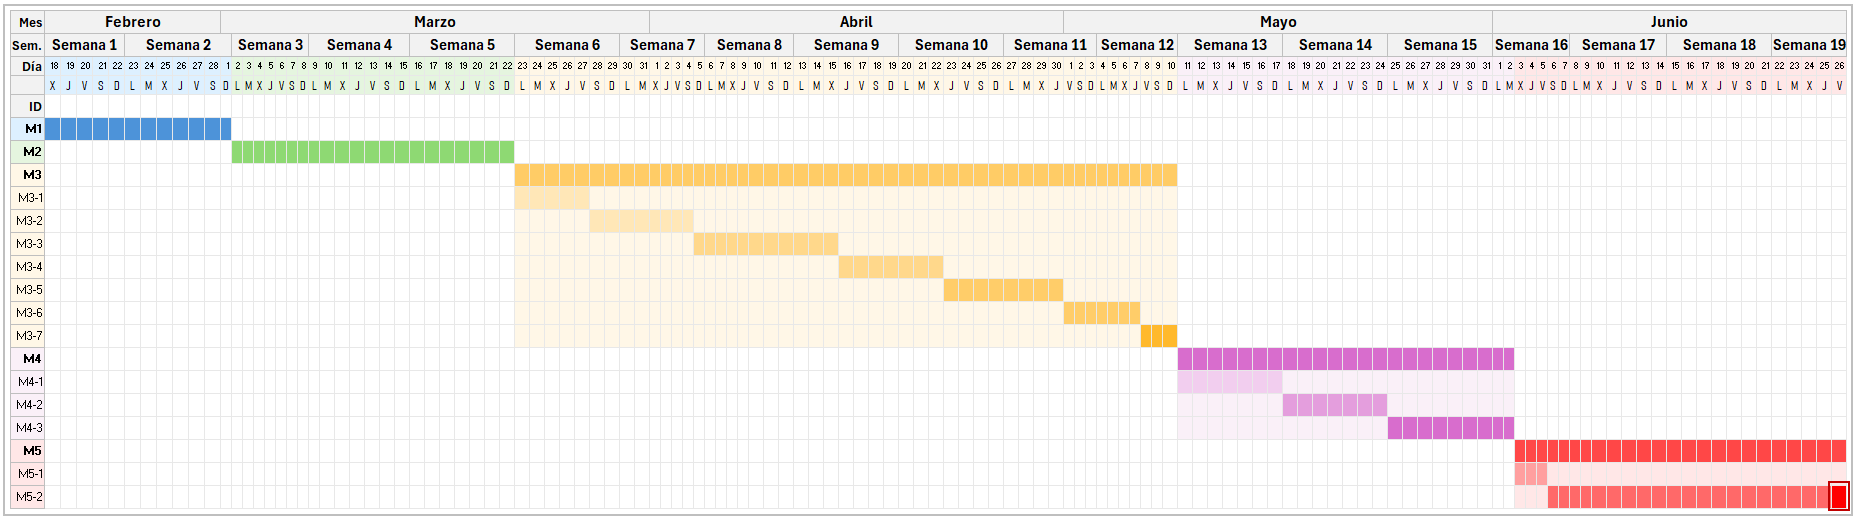
\includegraphics[width=1.1\textwidth]{images/planing.png}
\caption{Calendario de la planificación del proyecto (formato Gantt).}
\label{fig:planing}
\end{figure}


La planificación permite solapamientos controlados entre fases,
iniciando tareas como interpretabilidad o reconciliación jerárquica una
vez establecida una primera versión del modelo base. Esto optimiza el
tiempo disponible y reduce riesgos de acumulación de tareas en fases finales.

\newpage
\subsection{Gestión de riesgos del proyecto}

Se identifican los siguientes riesgos potenciales:

\begin{itemize}
\item
  \textbf{Coste computacional elevado del modelo LSTM}\\
  Probabilidad: Media\\
  Impacto: Alto\\
  Mitigación: uso de subconjuntos jerárquicos y reducción de
  dimensionalidad inicial.
\item
  \textbf{Dificultad en implementación de MinT}\\
  Probabilidad: Media\\
  Impacto: Medio\\
  Mitigación: priorizar Bottom-Up como método base garantizado.
\item
  \textbf{Rendimiento similar entre modelos sin diferencias
  significativas}\\
  Probabilidad: Media\\
  Impacto: Bajo\\
  Mitigación: enfocar el análisis en interpretabilidad y eficiencia
  computacional.
\item
  \textbf{Desviaciones en la planificación por complejidad técnica}\\
  Probabilidad: Media\\
  Impacto: Medio\\
  Mitigación: desarrollar primero un pipeline mínimo reproducible antes
  de optimizaciones avanzadas.
\item
  \textbf{Riesgo de data leakage en validación temporal\\
  }Probabilidad: Media\\
  Impacto: Alto\\
  Mitigación: validación walk-forward estricta y separación clara por
  horizonte.
\end{itemize}

La gestión de riesgos se integrará de forma dinámica en la planificación
temporal del proyecto. Cada hito técnico definido en la tabla de
planificación funcionará como punto de control para evaluar desviaciones
y activar medidas de mitigación, especialmente en las fases de modelado
y reconciliación jerárquica.

Cada riesgo será evaluado al final de su fase correspondiente, usando
los hitos técnicos como punto de control.

\newpage
\section{Impacto en sostenibilidad, ético-social y diversidad}

Desde la dimensión de sostenibilidad, una mejora en la precisión de los
modelos de predicción de demanda puede contribuir a reducir la
sobreproducción, el desperdicio de productos y los costes logísticos
asociados al transporte y almacenamiento, alineándose con objetivos de
eficiencia operativa y reducción del impacto ambiental.

Asimismo, se considerará la eficiencia computacional y energética de los
modelos desarrollados, analizando el impacto relativo de arquitecturas
más complejas como LSTM frente a modelos basados en árboles, en línea
con enfoques de inteligencia artificial sostenible.

En cuanto al comportamiento ético y responsabilidad social, el dataset
M5 se encuentra completamente anonimizado, sin incluir datos personales,
garantizando el respeto a la privacidad y el cumplimiento de normativas
de protección de datos. Además, se enfatiza que los modelos
desarrollados deben utilizarse como herramientas de apoyo a la toma de
decisiones y no como mecanismos automatizados excluyentes.

Finalmente, el uso de datasets públicos procedentes de plataformas
abiertas como Kaggle fomenta la accesibilidad, la igualdad de
oportunidades en investigación y la colaboración global, promoviendo la
diversidad en el desarrollo y evaluación de soluciones de inteligencia
artificial.

\newpage

\chapter{Estado del arte}

Aunque existen numerosos estudios que analizan modelos basados en
boosting, redes LSTM o técnicas de reconciliación jerárquica de forma
independiente, no es habitual encontrar trabajos que integren estos
enfoques dentro de un mismo marco metodológico. Este hecho justifica la
relevancia del presente trabajo, que propone una comparación entre
modelos basados en árboles y redes LSTM, incorporando técnicas de
reconciliación jerárquica mediante MinT e interpretabilidad mediante
SHAP.

La predicción de demanda en retail ha sido ampliamente estudiada debido
a su impacto en la planificación de inventarios, la gestión logística y
la toma de decisiones. Estos entornos presentan una elevada complejidad
estructural: miles de series temporales interrelacionadas, múltiples
niveles jerárquicos, estacionalidad, efectos de calendario y variaciones
derivadas de promociones o cambios de precio (\cite{hyndman2021}). 
Este contexto ha favorecido el uso de modelos capaces de manejar
grandes volúmenes de datos y capturar relaciones no lineales.

El dataset M5 Forecasting -- Walmart (\cite{makridakis2021})
constituye un benchmark relevante por su estructura jerárquica profunda,
granularidad diaria y diversidad de variables explicativas, permitiendo
comparar modelos estadísticos y de machine learning bajo un mismo marco.

\section{Predicción de demanda en retail: problemática y enfoques clásicos}

La demanda en retail está influida por múltiples factores simultáneos:
estacionalidad, tendencias, eventos, promociones, variaciones de precio
y diferencias entre tiendas o regiones, tal como se observa en distintos
enfoques de modelización de demanda\hl{.} La presencia de miles de
series con comportamientos heterogéneos ha impulsado el desarrollo de
modelos globales, capaces de aprender patrones compartidos entre
productos y tiendas (\cite{salinas2017}).

Los métodos univariantes como ARIMA o ETS han sido ampliamente
utilizados, pero presentan limitaciones al abordar estructuras
jerárquicas complejas y múltiples variables explicativas (\cite{hyndman2021}). Esta
limitación ha favorecido la adopción de modelos más flexibles y
escalables.

\emph{\textbf{\hl{Para contextualizar esta transición, es necesario
detallar brevemente el funcionamiento de los modelos clásicos. ARIMA
modela la serie temporal como una combinación lineal de tres
componentes: (i) un término autorregresivo (AR) basado en rezagos de la
propia serie, (ii) un término de diferenciación (I) que busca garantizar
estacionariedad y (iii) un componente de medias móviles (MA) que
incorpora errores pasados. Este enfoque asume relaciones lineales y una
estructura temporal relativamente simple.}}}

\emph{\textbf{\hl{SARIMA extiende ARIMA incorporando términos
estacionales adicionales (AR, I y MA estacionales), lo que permite
capturar patrones repetitivos como los semanales o mensuales. Sin
embargo, ambos modelos presentan limitaciones importantes: requieren
estacionariedad, no integran de forma natural múltiples variables
explicativas, no capturan relaciones no lineales y escalan mal cuando se
trabaja con miles de series simultáneamente.}}}

\emph{\textbf{\hl{Estas limitaciones motivaron la adopción de modelos
más flexibles y escalables, como los métodos de gradient boosting y las
redes LSTM, que se desarrollan en las subsecciones siguientes. En
particular, estos enfoques permiten modelar relaciones no lineales,
incorporar múltiples variables explicativas y escalar de forma eficiente
a conjuntos de datos con un gran número de series temporales, superando
algunas de las restricciones inherentes a los modelos clásicos.}}}

\subsection{Modelos de Gradient Boosting para forecasting}

Los modelos basados en árboles, como Random Forest (\cite{Breiman2001}),
XGBoost (\cite{chen2016xgboost}) y LightGBM (\cite{ke2017lightgbm}), presentan
un rendimiento destacado en datos tabulares de alta dimensionalidad. En
la competición M5, los modelos de gradient boosting fueron predominantes
entre las soluciones mejor posicionadas (\cite{makridakis2021}).

La literatura indica que, combinados con un feature engineering adecuado
-- lags, ventanas móviles, variables de calendario y de precio --,
pueden ofrecer un rendimiento competitivo frente a modelos más complejos
como las redes neuronales recurrentes (\cite{hewamalage2021}). Esto
respalda su uso como base en el presente trabajo.

\emph{\textbf{\hl{Desde un punto de vista técnico, los modelos de
gradient boosting construyen árboles de decisión de manera secuencial:
cada nuevo árbol se entrena para corregir los errores residuales del
árbol anterior. Este proceso iterativo permite capturar relaciones no
lineales y manejar interacciones complejas entre variables sin necesidad
de especificarlas explícitamente.}}}

\emph{\textbf{\hl{Este enfoque se basa en un esquema de aprendizaje
aditivo, en el que cada nuevo modelo se centra en corregir los errores
acumulados, optimizando de forma iterativa una función de pérdida
definida sobre el conjunto de entrenamiento.}}}

\emph{\textbf{\hl{Modelos como XGBoost y LightGBM incorporan técnicas
avanzadas de regularización, manejo eficiente de memoria, histogramas
para acelerar la búsqueda de divisiones y estrategias de reducción del
sobreajuste. Estas características los hacen especialmente adecuados
para problemas de forecasting con grandes volúmenes de datos, múltiples
variables explicativas y estructuras jerárquicas profundas.}}}

\emph{\textbf{\hl{Su principal limitación es que no modelan
explícitamente la dependencia temporal de largo plazo, ya que trabajan
sobre features tabulares generadas manualmente (lags, ventanas,
calendarios). Esto ha impulsado el uso de modelos secuenciales como las
LSTM.}}}

\subsection{Redes LSTM y modelos profundos para predicción de demanda}

Las redes neuronales recurrentes, en particular las LSTM (\cite{hochreiter1997}), 
están diseñadas para capturar dependencias
temporales de largo plazo sin necesidad de ingeniería manual intensiva.
Gracias a esta arquitectura, las LSTM son capaces de capturar
dependencias temporales complejas y patrones de largo plazo en las
series, reduciendo la necesidad de ingeniería manual de variables basada
en retardos.

\emph{\textbf{\hl{Las LSTM incorporan una arquitectura basada en
``celdas de memoria'' y tres puertas (entrada, olvido y salida) que
regulan qué información se mantiene, cuál se descarta y cuál se
transmite a pasos futuros. Esta estructura permite mitigar el problema
del desvanecimiento del gradiente y facilita el aprendizaje de patrones
temporales complejos.}}}

\emph{\textbf{\hl{A pesar de estas ventajas, presentan limitaciones
relevantes: requieren grandes volúmenes de datos limpios, son sensibles
a la configuración de hiperparámetros, tienen un coste computacional
elevado y ofrecen menor interpretabilidad que los modelos basados en
árboles. En la competición M5, su rendimiento fue inferior al de los
modelos boosting, lo que ha generado debate sobre su aplicabilidad en
entornos productivos.}}}

\emph{\textbf{\hl{Su inclusión en este trabajo permite comparar enfoques
tabulares y secuenciales bajo un mismo marco metodológico, evaluando no
solo la precisión, sino también la eficiencia computacional y la
interpretabilidad.}}}

\section{Series temporales jerárquicas y reconciliación}

La estructura jerárquica de los datos constituye un elemento central del
problema. En el caso de Walmart, las ventas pueden agregarse por estado,
tienda, categoría o producto, generando distintos niveles que deben
mantener coherencia entre sí.

Los enfoques tradicionales como Bottom-Up, Top-Down o Middle-Out
(\cite{hyndman2011}) permiten agregar o desagregar predicciones, pero
no consideran la correlación entre errores de predicción.

Para abordar esta limitación, \cite{wickramasuriya2019} proponen MinT
(Minimum Trace), que ajusta las predicciones base mediante una
combinación lineal que minimiza la traza de la matriz de covarianzas de
los errores, lo que equivale a minimizar la varianza total de los
errores reconciliados bajo una combinación lineal óptima. Este enfoque
produce predicciones más eficientes y coherentes, especialmente en
jerarquías profundas como la del M5. Por ello, en este trabajo se emplea
MinT como técnica principal, complementada con Bottom-Up como
referencia.

La necesidad de garantizar coherencia jerárquica requiere modelos
capaces de generar predicciones base robustas.

\section{Interpretabilidad en forecasting: valores SHAP}

La interpretabilidad constituye un requisito clave en aplicaciones
empresariales. Los valores SHAP (\cite{lundberg2017shap}) se han
consolidado como una herramienta estándar para explicar modelos
complejos, especialmente los basados en árboles. SHAP permite analizar
la contribución marginal de cada variable, identificar patrones y
evaluar la estabilidad del modelo. En este trabajo se aplica sobre las
predicciones base, dado que la reconciliación constituye un ajuste
posterior.

\emph{\textbf{\hl{Además de su utilidad técnica, la interpretabilidad
desempeña un papel fundamental en la adopción real de modelos de
forecasting dentro de organizaciones retail. En estos entornos, los
equipos de negocio necesitan comprender por qué un modelo predice un
aumento o disminución de la demanda, especialmente cuando las decisiones
afectan a inventario, promociones o asignación de recursos.}}}

\emph{\textbf{\hl{Los valores SHAP permiten identificar qué variables
impulsan la predicción en cada instante, facilitando la detección de
patrones relevantes como efectos de precio, estacionalidad o impacto de
promociones. Esta información puede emplearse para diseñar campañas
comerciales más efectivas, ajustar estrategias de pricing o priorizar
productos con alta sensibilidad a determinados factores.}}}

\emph{\textbf{Asimismo, SHAP favorece la comunicación entre perfiles
técnicos y no técnicos, reduciendo la percepción de ``caja negra''
asociada a modelos complejos. Esto incrementa la confianza en el sistema
de forecasting y facilita su integración en procesos de toma de
decisiones operativas y estratégicas.}}

\emph{\textbf{En entornos retail, donde las decisiones deben
justificarse ante múltiples áreas, la interpretabilidad resulta
especialmente relevante para garantizar la adopción efectiva de los
modelos y asegurar que las predicciones puedan ser comprendidas,
validadas y utilizadas en la práctica.}}

\section{La competición M5 Forecasting y trabajos relacionados}

El dataset M5 ha dado lugar a numerosos trabajos académicos y soluciones
industriales.

Aunque existen trabajos centrados en modelos boosting, otros en LSTM y
algunos en reconciliación jerárquica, no es habitual encontrar un
enfoque que integre estos elementos en un mismo pipeline orientado a la
comparación sistemática.

\emph{\textbf{\hl{Las soluciones mejor posicionadas compartieron varios
elementos clave: (i) el uso de modelos globales entrenados sobre todas
las series simultáneamente, lo que permitió capturar patrones comunes
entre productos y tiendas; (ii) un feature engineering muy intensivo,
incluyendo lags, medias móviles, indicadores de calendario, variables de
precio y variables derivadas de eventos; y (iii) una optimización
exhaustiva de hiperparámetros mediante técnicas como grid search o
Bayesian optimization.}}}

\emph{\textbf{\hl{El equipo ganador (1st place), según la documentación oficial de Kaggle, utilizó un modelo LightGBM global con un conjunto de más de 300 variables derivadas y obtuvo un WRMSSE de 0.520. El segundo y tercer clasificado también emplearon modelos boosting (LightGBM o CatBoost), con WRMSSE en rangos muy próximos al ganador ($\sim$0.52-0.53), lo que evidencia que las diferencias entre las mejores soluciones fueron mínimas y dependieron principalmente de ajustes finos en la ingeniería de características.}}}

\emph{\textbf{\hl{El análisis del repositorio oficial de la competición
muestra que las redes neuronales profundas, incluidas las LSTM,
obtuvieron resultados inferiores en la mayoría de los casos, debido a su
mayor complejidad, sensibilidad al preprocesado y dificultad para
capturar patrones idiosincráticos en miles de series cortas. Este
comportamiento coincide con los hallazgos del paper oficial de la M5,
que destaca el dominio de los modelos boosting en contextos de
forecasting retail con estructuras jerárquicas profundas.}}}

\emph{\textbf{A continuación, se presenta un resumen estructurado de las
soluciones mejor clasificadas en la competición, incluyendo sus
principales características y métricas, que servirán como referencia
comparativa para los experimentos desarrollados en este trabajo (Tabla 2).}}

\begin{longtable}{p{1.6cm} !{\vrule width 0.1pt} p{2.4cm} !{\vrule width 0.1pt} p{2.5cm} !{\vrule width 0.1pt} p{3.5cm} !{\vrule width 0.1pt} p{2.2cm} !{\vrule width 0.1pt} p{1.5cm}}


\toprule
\textbf{Posición} & \textbf{Equipo / Autor} & \textbf{Modelo principal} & \textbf{Características clave} & \textbf{WRMSSE} & \textbf{Fuente} \\
\midrule
\endfirsthead

\toprule
\textbf{Posición} & \textbf{Equipo / Autor} & \textbf{Modelo principal} & \textbf{Características clave} & \textbf{WRMSSE} & \textbf{Fuente} \\
\midrule
\endhead

\textbf{1º} & Kailex & LightGBM global & Feature engineering intensivo (>300 variables), modelo global, tuning exhaustivo & 0.52 & \cite{kailex2020} \\
\midrule
\textbf{2º} & Matthias & LightGBM & Ventanas temporales optimizadas, variables de precio, regularización avanzada & $\sim 0.52$--$0.53$ & \cite{matthias2020} \\
\midrule
\textbf{3º} & Rob Mulla (Robikscube) & LightGBM + modelos globales & Feature engineering profundo, validación cruzada por series & $\sim 0.53$ & \cite{mulla2020} \\
\midrule
Top 10 & Varios & LightGBM / CatBoost & Variaciones en ingeniería de variables y tuning & 0.52--0.54 & \cite{m5competition2020} \\
\midrule
Paper oficial & Makridakis et al. (2020) & --- & Análisis de resultados y patrones comunes & --- & \cite{makridakis2021} \\
\bottomrule

\end{longtable}

\textbf{Tabla 2.} Resumen de las soluciones mejor clasificadas en la competición M5 (Accuracy Track).   

\newpage
\section{Síntesis y relevancia del trabajo}

La literatura muestra que la predicción de demanda en estructuras
jerárquicas requiere modelos capaces de manejar alta dimensionalidad,
capturar patrones temporales y mantener coherencia entre niveles. 
Se observa un claro predominio de enfoques centrados de forma aislada en modelos boosting, modelos profundos o técnicas de reconciliación jerárquica. Sin embargo, estos trabajos rara vez abordan de forma conjunta la interacción entre precisión predictiva, coherencia jerárquica, coste computacional e interpretabilidad dentro de un mismo marco experimental.
En este contexto, el presente trabajo propone una aproximación integradora que combina estos elementos en un único pipeline reproducible, permitiendo evaluar de forma sistemática no solo el rendimiento predictivo, sino también las implicaciones prácticas de cada enfoque en términos de escalabilidad, interpretabilidad y aplicabilidad en entornos reales de retail.
La reconciliación jerárquica mediante MinT se
consolida como un componente clave para asegurar coherencia estructural,
mientras que SHAP facilita la interpretación de modelos complejos y su
adopción por parte de perfiles no técnicos.

La revisión de la competición M5 confirma el predominio de los modelos
boosting -- especialmente LightGBM -- en contextos de forecasting retail
con jerarquías profundas. En línea con lo observado en la competición
M5, las soluciones mejor clasificadas comparten patrones claros: uso de
modelos globales, feature engineering intensivo y optimización
exhaustiva de hiperparámetros. Estas estrategias permitieron alcanzar
valores WRMSSE en el rango \textbf{0.52-0.53}, que constituyen el
\textbf{benchmark de referencia} para evaluar el rendimiento de los
modelos desarrollados en este trabajo.

A pesar de estos avances, la literatura carece de un análisis integrado
que combine modelos boosting, redes LSTM, reconciliación jerárquica e
interpretabilidad dentro de un mismo marco metodológico. Este trabajo
aborda dicho vacío mediante una comparación sistemática que evalúa
precisión, coherencia jerárquica, coste computacional e
interpretabilidad en el contexto del dataset M5. Esta aproximación
permite no solo contrastar el rendimiento de los distintos modelos, sino
también situar los resultados obtenidos frente a los estándares
establecidos por las soluciones más exitosas de la competición.

\addcontentsline{toc}{section}{Bibliografía}
\bibliographystyle{plainurl}
\bibliography{references}

\end{document}

